\documentclass[tikz]{standalone}
\usetikzlibrary{arrows}
\tikzset{
  treenode/.style = {align=center, inner sep=1pt, text centered,
    font=\sffamily},
  arn_b/.style = {treenode, circle, white, font=\sffamily\bfseries, draw=black,
    fill=black, text width=1.5em},% arbre rouge noir, noeud noir
  arn_r/.style = {treenode, circle, red, draw=red, 
    text width=1.5em, very thick},% arbre rouge noir, noeud rouge
  arn_x/.style = {treenode, rectangle, draw=black,
    minimum width=0.5em, minimum height=0.5em}% arbre rouge noir, nil
}

\begin{document}
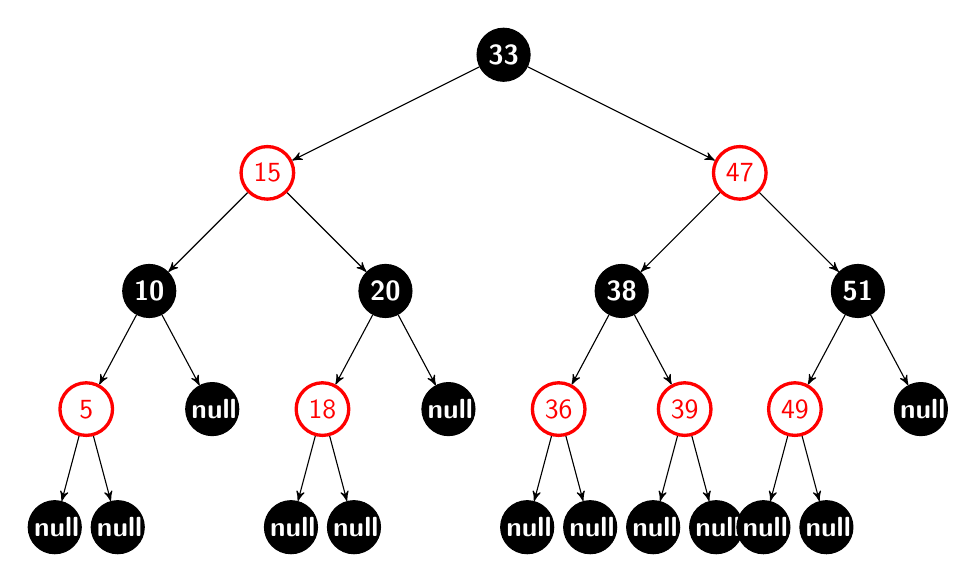
\begin{tikzpicture}[->,>=stealth',level/.style={sibling distance = 6cm/#1,
  level distance = 1.5cm}, level 3/.style={sibling distance = 1.6cm}, level 4/.style={sibling distance = 0.8cm}] 
\node [arn_b] {33}
    child{ node [arn_r] {15} 
            child{ node [arn_b] {10} 
            	child{ node [arn_r] {5}
                         child{ node [arn_b] {null}}
                         child{ node [arn_b] {null}}} 
				child{ node [arn_b] {null} }
            }
            child{ node [arn_b] {20}
							child{ node [arn_r] {18}
                            child{ node [arn_b] {null}}
                            child{ node [arn_b] {null}}}
							child{ node [arn_b] {null}}
            }                            
    }
    child{ node [arn_r] {47}
            child{ node [arn_b] {38} 
							child{ node [arn_r] {36}
                            child{ node [arn_b] {null}}
                            child{ node [arn_b] {null}}}
							child{ node [arn_r] {39}
                            child{ node [arn_b] {null}}
                            child{ node [arn_b] {null}}}
            }
            child{ node [arn_b] {51}
							child{ node [arn_r] {49}
                            child{ node [arn_b] {null}}
                            child{ node [arn_b] {null}}}
							child{ node [arn_b] {null}}
            }
		}; 
\end{tikzpicture}
\end{document}

